\documentclass[twocolumn]{article}
\usepackage[utf8]{inputenc}
\usepackage{listings}
\usepackage{geometry}
\usepackage{graphicx}
\usepackage{multicol}
\usepackage{amsmath}
\usepackage{cite}
\usepackage{float}
\usepackage{enumitem}
\usepackage[colorlinks=true,linkcolor=black,urlcolor=blue,citecolor=blue]{hyperref}
\usepackage{tabularx}
\geometry{a4paper, margin=2cm}

\title{\huge\bfseries Makine Öğrenmesi Modelleri Kullanarak Hava Durumu Analizi ve Sınıflandırılması
}

\author{
	Ogün ATALAY\\
	Bilgisayar Mühendisliği 3.Sınıf\\
	Kahramanmaraş Sütçü İmam Üniversitesi\\
	Kahramanmaraş, Türkiye\\
	\texttt{ogun.atalay33@gmail.com}
}
\date{\today}

\begin{document}
	
	\maketitle
	
	\textbf{Özet:} \\
	Hava durumu analizi ve sınıflandırması, tarımın verimliliğinden ulaşımın güvenliğine, afet yönetiminden enerji planlamasına kadar geniş bir yelpazede hayati öneme sahip olan bir alanı temsil eder. Bu bağlamda, hava durumu verileri üzerinde yapılan bu proje, veri analizi ve makine öğrenimi modellemesi kullanarak hava durumu koşullarını sınıflandırmayı amaçlamaktadır. Proje, veri setinin keşfedilmesi, görselleştirilmesi ve ön işlenmesi aşamalarını içermektedir. Ardından, farklı makine öğrenimi algoritmaları, sıcaklık, yağış miktarı ve rüzgar hızı gibi özelliklere dayanarak hava durumu koşullarını sınıflandırmak için eğitilmiş ve test edilmiştir. 
	
	\textbf{Anahtar Kelimeler:} Hava durumu, veri analizi, makine öğrenmesi, sınıflandırma, sıcaklık, yağış miktarı, rüzgar. 
	
	\textbf{Abstract:} \\
	The analysis and classification of weather conditions represent a vital area that encompasses a wide range of importance, from agricultural productivity to transportation safety, disaster management, and energy planning. In this context, this project conducted on weather data aims to classify weather conditions using data analysis and machine learning modeling. The project includes stages of data exploration, visualization, and preprocessing. Subsequently, different machine learning algorithms have been trained and tested to classify weather conditions based on features such as temperature, precipitation, and wind speed.
	
	\textbf{Keywords:} Weather, data analysis, machine learning, classification, temperature, precipitation, wind 
	
	\section{GİRİŞ}
	
	Bu proje, gerçek dünya hava durumu verileri üzerinde kapsamlı bir veri analizi ve modelleme yaklaşımını benimseyerek, çeşitli makine öğrenimi tekniklerini kullanarak hava koşullarını tahmin etmeyi amaçlayan bir araştırma çalışmasıdır. Toplanan veri setinde yer alan minimum ve maksimum sıcaklık, yağış miktarı ve rüzgar hızı gibi hava durumu özellikleri, farklı makine öğrenimi algoritmalarıyla değerlendirilerek en etkili tahminleme modelinin belirlenmesi hedeflenmektedir. Bu çalışma, makine öğrenimi yöntemlerinin pratik kullanımını göstermenin yanı sıra, hava durumu tahminlemesi üzerine genel bir çerçeve sunmayı amaçlamaktadır, böylelikle benzer uygulamalarda da bu metodolojinin kullanılmasına ışık tutmaktadır.
	
	\section{LİTERATÜR ÖZETİ}
	
	Hava durumu analizi ve sınıflandırması, çeşitli algoritma ve yapay zekâ metotları ile birden fazla giriş parametresi kullanılarak gerçekleştirilebilir. Yapay zekâ, karmaşık verilerin daha iyi temsil edilmesini ve yorumlanmasını sağlayan bir öğrenme yöntemidir \cite{hosny2018artificial}.
	
	Bu projede çeşitli makine öğrenmesi modelleri kullanılmıştır. Makine öğrenmesi; denetimli, denetimsiz ve takviyeli olmak üzere üç ayrı kategoride sınıflandırılmaktadır \cite{greenspan2016guest}. Denetimli öğrenme genellikle verinin bir veya daha fazla kategoriye ayrılarak sınıflandırılması için kullanılırken, denetimsiz öğrenme ise veri setindeki değişkenler ve arasındaki ilişkiyi keşfetmeye odaklanmaktadır \cite{johnson2018artificial}. Takviyeli öğrenme ise, bir sistemin davranışsal kararlar verme yeteneğini geliştirmek için dünya ile etkileşime girerek kazanılan deneyimi ve değerlendirici geri bildirimi kullanmakla ilgili bir makine öğrenim alanıdır \cite{littman2015reinforcement} . Projede denetimli makine öğrenmesi modellerinden faydalanılmıştır: Logistic Regression, Random Forest Classifier, Gradient Boosting Classifier, K-Nearest Neighbors Classifier, Support Vector Classifier (SVC), Decision Tree Classifier. 
	
	\section{VERİ SETİ VE YÖNTEM}
	
	\subsection{Veri Seti}
	Bu projenin veri seti, bir şehirdeki 2012-2015 yılı boyunca günlük hava durumu verilerini içermektedir. Veri setindeki değişkenler şu şekildedir \cite{ananthr1_weather_prediction} :
	\begin{itemize}
		\item \textbf{date:} Ölçülen tarih (yıl-ay-gün formatında).
		\item \textbf{precipitation:} Günlük yağış miktarı (inç cinsinden).
		\item \textbf{temp\_max:} Günlük maksimum sıcaklık (°C cinsinden).
		\item \textbf{temp\_min:} Günlük minimum sıcaklık (°C cinsinden).
		\item \textbf{wind:} Günlük rüzgar hızı (mil/saat cinsinden).
		\item \textbf{weather:} Günlük hava durumu (örneğin, yağmur, kar, güneş, vb.).
	\end{itemize}
	Bu veri seti, hava durumu koşullarının farklı özelliklerini içerir ve her bir günün belirli bir hava durumu kategorisine atanmış bir etiketi bulunmaktadır. Bu etiketler, hava durumu tahmin modelinin eğitilmesi ve test edilmesi için kullanılacaktır.
	
	\subsection{Yöntem}
	Proje yöntemi olarak, veri seti üzerinde çeşitli makine öğrenimi sınıflandırma modelleri eğitilerek, günlük hava durumu koşullarının tahmin edilmesi amaçlanmaktadır. İşlem adımları şu şekildedir:
	\begin{enumerate}
		\item \textbf{Veri Keşfi ve Görselleştirme:} Veri seti görselleştirilerek (histogramlar, çizgi grafikleri, vs.) hava durumu özelliklerinin dağılımı ve değişimi incelenecek ve anlaşılacaktır.
		\item \textbf{Veri Ön İşleme:} Veri seti makine öğrenimi modeline uygun hale getirilecektir. Bu adımda eksik verilerin doldurulması, kategorik değişkenlerin kodlanması gibi işlemler gerçekleştirilecektir.
		\item \textbf {Modelleme:} Farklı sınıflandırma modelleri (Logistic Regression, Random Forest Classifier, Gradient Boosting Classifier, K-Nearest Neighbors Classifier, Support Vector Classifier (SVC), Decision Tree Classifier) kullanılarak veri seti eğitilecek ve test edilecektir.
		\item \textbf{Performans Değerlendirmesi:} Her modelin performansı değerlendirilecek ve en iyi performansı sergileyen model seçilecektir. Bu süreçte, model performansını değerlendirmek için doğruluk, F1 skoru ve diğer sınıflandırma metrikleri kullanılacaktır.
		
		\[
		F1 \text{ Skoru} = 2 \times \frac{\text{Precision} \times \text{Recall}}{\text{Precision} + \text{Recall}}
		\]
		
		\item \textbf {Sonuçların İncelenmesi ve Yorumlanması:} En iyi model seçildikten sonra, sonuçlar incelenecek ve elde edilen bulgular yorumlanarak bir rapor hazırlanacaktır.
	\end{enumerate}
	Bu yöntem, günlük hava durumu tahmininde kullanılan makine öğrenimi tekniklerini uygulayarak, veri setindeki bilgilerin kullanışlılığını artırmayı ve hava durumu tahminlerinin doğruluğunu artırmayı amaçlamaktadır.
	
	\section{KULLANILAN MODELLER} 
	\subsection{Logistic Regression}
	
	\begin{itemize}
		\item \textbf{Kullanım Alanı:} Lojistik regresyon, ikili sınıflandırma problemlerinde kullanılan bir modeldir. Bu projede, günlük hava durumu koşullarının belirli bir kategoriye (örneğin, yağmur, kar, güneş) atanması için lojistik regresyon modeli kullanılabilir.
		\item \textbf{Veri Hazırlığı:} Lojistik regresyon modeline veri seti, bağımsız değişkenler (temp\_min, temp\_max, precipitation, wind) ve bağımlı değişken (weather) olarak ayrılır. Bağımlı değişken, kategorik olarak kodlanır.
		\item \textbf{Model Eğitimi:} Veri seti, eğitim ve test setlerine ayrılır. Ardından, lojistik regresyon modeli eğitim veri seti üzerinde eğitilir. Model, giriş özellikleri ile bağımlı değişken arasındaki ilişkiyi öğrenir.
		\item \textbf{Model Tahmini:} Eğitilen model, test veri seti üzerinde kullanılarak tahminler yapar. Model, giriş özelliklerine dayanarak her bir gözlemin hangi hava durumu kategorisine ait olduğunu tahmin eder.
		\item \textbf{Performans Değerlendirmesi:} Modelin performansı, doğruluk (accuracy), hassasiyet (precision), özgüllük (recall) ve F1 skoru gibi metrikler kullanılarak değerlendirilir. Modelin doğruluğu, gerçek ve tahmin edilen hava durumu kategorileri arasındaki uyumu ölçer.
		\item \textbf{Sonuçlar ve Yorumlar:} Modelin performansı incelenir ve yorumlanır. Eğer model yeterince iyi performans gösterirse, günlük hava durumu koşullarının tahmininde kullanılabilir. Ayrıca, modelin güçlü ve zayıf yönleri hakkında bir değerlendirme yapılır ve iyileştirmeler veya değişiklikler önerilebilir.
		
	\end{itemize}
	
	\textbf{Logistic Regression Formülü:} \cite{omu_logistic_regression}
	
	\[ P(Y=1|X) = \frac{1}{1 + e^{-(\beta_0 + \beta_1 X_1 + \beta_2 X_2 + \ldots + \beta_n X_n)}} \]
	
	\textbf{Logistic Regression İçin F1 Skoru Hesaplama Formülü:}
	
	\[ F1 = 2 \times \frac{\text{Precision} \times \text{Recall}}{\text{Precision} + \text{Recall}} \]
	
	\[ \text{Precision (Hassasiyet):} \quad \frac{TP}{TP + FP} \]
	
	\[ \text{Recall (Özgüllük):} \quad \frac{TP}{TP + FN} \]
	
	Burada, \(TP\) doğru pozitif sayısını, \(FP\) yanlış pozitif sayısını ve \(FN\) yanlış negatif sayısını temsil eder.
	
	
	\begin{flushleft}
		\subsection{Random Forest Classifier}
		\begin{description}
			\item\textbf{Çalışma Prensibi:} Random Forest, birden fazla karar ağacını (decision tree) bir araya getirir ve her bir ağacın tahminini alarak çoğunluk oyuyla bir sonuç verir. Her karar ağacı, rastgele seçilen özellikler alt kümesi üzerinde eğitilir ve veri setinin bir alt kümesi üzerinde tahmin yapar. Bu şekilde, birçok karar ağacının tahminleri birleştirilerek daha doğru ve genelleştirilebilir bir tahmin elde edilir.
			
			\item\textbf{Veri Hazırlığı:} İlk adımda, hava verileri okunur ve gereksiz sütunlar düşürülerek, hava durumu etiketleri sayısal değerlere dönüştürülür. Bu adımlar veri setinin hazırlanmasını sağlar.
			
			\item\textbf{Bağımsız ve Bağımlı Değişkenlerin Belirlenmesi:} Makine öğrenimi modelinin eğitilmesi için bağımsız değişkenler (X) ve bağımlı değişken (y) belirlenir. Bağımsız değişkenler, hava durumunu tahmin etmek için kullanılan özellikleri içerirken, bağımlı değişken hava durumu etiketlerini içerir.
			
			\item\textbf{Eğitim ve Test Setlerinin Oluşturulması:} Veri seti, eğitim ve test setlerine ayrılır. Bu, modelin eğitim verileri üzerinde öğrenmesini ve ardından test verileri üzerinde performansını değerlendirmesini sağlar.
			
			\item\textbf{Modelinin Oluşturulması ve Eğitilmesi:} RandomForestClassifier sınıfından bir model oluşturulur ve eğitim verileriyle eğitilir. Bu adımda, model hava verilerini kullanarak hava durumunu tahmin etmeyi öğrenir.
			
			\item\textbf{Çapraz Doğrulama:} Modelin performansını doğrulamak için çapraz doğrulama yapılır. Bu adım, modelin genelleme yeteneğini değerlendirmeye yardımcı olur ve aşırı uyumu önler.
			
			\item\textbf{Sonuçların Raporlanması:} Çapraz doğrulama sonuçları, modelin performansını belirlemek için kullanılır. Bu sonuçlar genellikle doğruluk (accuracy) değeri olarak raporlanır ve farklı modeller arasındaki karşılaştırmalar yapılabilir.
		\end{description}
		
		\subsection{Gradient Boosting Classifier}
		\begin{description}
			\item \textbf {Çalışma Prensibi:} Gradient Boosting Classifier, bir ensemble learning tekniği olan gradient boosting yöntemini kullanarak bir dizi zayıf öğreniciyi (genellikle karar ağaçları) bir araya getirerek bir sınıflandırma modeli oluşturur. Gradient boosting, bir önceki ağacın hatalarını düzeltmek için bir sonraki ağacı eğitmeye odaklanır.
			
			\item \textbf{İşleyişi:}
			
			
			\item \textbf{Başlangıç Modeli:} İlk olarak, veri seti üzerinde bir başlangıç modeli oluşturulur. Bu başlangıç modeli genellikle veri setinin sınıf dağılımı üzerinden tahminler yapar.
			\item \textbf{Hata Tespiti:} Her bir örnek için gerçek sınıf ile model tarafından yapılan tahmin arasındaki hata hesaplanır. Bu hata, gerçek sınıf ile tahmin edilen sınıf arasındaki fark olarak ölçülür.
			\item \textbf{Yeni Ağaç Oluşturma:} Hataları minimize etmek için yeni bir karar ağacı oluşturulur. Bu karar ağacı, hatalar üzerine odaklanarak eğitilir. Önceki ağaçların hatalarını düzeltmek için, yeni ağaç örneklerin özelliklerine dayalı olarak oluşturulur.
			\item \textbf{Ağırlıklandırma:} Yeni oluşturulan ağaç, bir önceki ağaçla birleştirilir ve birlikte kullanılır. Ancak, her bir ağacın katkısı ağırlıklandırılarak, daha fazla dikkat edilmesi gereken ağaçlar vurgulanır.
			\item \textbf{Adım Adım İterasyon:} Bu işlem, belirlenen bir iterasyon sayısına veya belirli bir hata eşiğine ulaşılana kadar tekrarlanır. Her iterasyonda, bir sonraki ağaç önceki ağaçların hatalarını minimize etmek için eğitilir.
			\item \textbf{Tahmin:} Son olarak, tüm ağaçların katkısı birleştirilir ve birlikte kullanılarak, bir giriş örneğinin sınıfını belirlemek için tahminler yapılır. Tahminler genellikle bir sınıf etiketi veya olasılık değeri olarak verilir.
			
		\end{description}
	\end{flushleft}
	
	
	\subsection{K-Nearest Neighbors Classifier}
	
	K-Nearest Neighbors (KNN) Sınıflandırıcısı, basit ve etkili bir makine öğrenimi algoritmasıdır. KNN, sınıflandırma problemlerinde ve regresyon problemlerinde kullanılabilir, ancak genellikle sınıflandırma için tercih edilir.
	
	KNN'nin çalışma mantığı şu adımlardan oluşur:
	
	\begin{enumerate}
		\item \textbf{Eğitim Aşaması:}
		
		Eğitim veri seti, özellikler (bağımsız değişkenler) ve hedef değişkenler (bağımlı değişkenler) olarak ayrılır. KNN algoritması, eğitim veri setindeki örnekleri depolar, ancak önceden eğitim yapmaz.
		
		\item \textbf{Tahmin Aşaması:}
		
		Yeni bir veri noktası geldiğinde, algoritma bu veri noktasının etrafındaki en yakın \textit{k} komşuyu bulur. En yakın \textit{k} komşuların etiketlerini (sınıflarını) inceleyerek, verilen veri noktasının sınıfını belirler. Sınıf belirleme işlemi genellikle çoğunluk oyu ilkesine dayanır: Yani, en yakın komşuların sınıfları arasında hangi sınıf daha fazlaysa, yeni veri noktası o sınıfa atanır.
		
		\item \textbf{Model Parametreleri:}
		
		KNN algoritmasının en önemli parametresi, komşu sayısıdır (\textit{k}). \textit{k}, genellikle tek sayı olarak seçilir, böylece oy kullanırken eşitlik durumunda çoğunluk sağlanır.
		
		\item \textbf{Uzaklık Ölçümü:}
		
		KNN'de en yaygın kullanılan uzaklık metrikleri Öklid mesafesi ve Manhattan mesafesidir. Ancak, kullanım durumuna göre farklı uzaklık ölçüleri de kullanılabilir.
		
		\textbf{KNN Öklid Mesafesi:} \cite{medium_knn}
		
		K-Nearest Neighbors (KNN) algoritması için birkaç önemli formül vardır. En yaygın kullanılanı, veri noktaları arasındaki mesafeyi hesaplamak için kullanılan Öklid mesafesi formülüdür. Bu formül, iki nokta arasındaki düz bir hattın uzunluğunu verir ve genellikle KNN algoritmasında komşuları belirlemek için kullanılır.
		
		\textbf{Öklid Mesafesi:} 
		
		\[
		d(\mathbf{x}, \mathbf{y}) = \sqrt{(t_{\text{min}x} - t_{\text{min}y})^2 + (t_{\text{max}x} - t_{\text{max}y})^2} + 
		\]
		\[
		\begin{aligned}
			&\quad \sqrt{(p_x - p_y)^2 + (w_x - w_y)^2}
		\end{aligned}
		\]
		
		\[
		\begin{aligned}
			& t max: && \text{Maksimum Sıcaklık} \\
			& t min: && \text{Minimum Sıcaklık} \\
			& p: && \text{Tahmin} \\
			& w: && \text{Rüzgar} \\
			& \mathbf{x} \text{ ve } \mathbf{y}: && \text{İki farklı veri noktası}
		\end{aligned}
		\]
	\end{enumerate}
	
	\subsection{Decision Tree}
	
	Bu algoritma, veri setini küçük ve hatta daha küçük parçalara bölerek geliştirilir. Bir karar düğümü bir veya birden fazla dallanma içerebilir. İlk düğüme kök düğüm (root node) denir. Bir karar ağacı hem kategorik hem de sayısal verilerden oluşabilir. \cite{decision_tree_id3}
	
	Decision Tree algoritmasının temel bileşenleri ve nasıl çalıştığına dair bazı önemli noktalar:
	
	\textbf{Temel Bileşenler}
	
	\begin{itemize}
		\item \textbf{Kök Düğüm (Root Node):} Karar ağacının başlangıç düğümüdür. Tüm veri seti bu düğüme gelir.
		\item \textbf{Dahili Düğümler (Internal Nodes):} Kök düğüm dışındaki düğümlerdir. Bunlar, bir özellik (feature) üzerinde bir karar kuralı içerir ve veri setini alt kümelere böler.
		\item \textbf{Kenarlar (Edges):} Düğümleri birbirine bağlayan çizgilerdir. Her kenar, bir özellik değeri için bir şarta karşılık gelir.
		\item \textbf{Yaprak Düğümler (Leaf Nodes):} Karar ağacının en alt düzeyinde bulunan düğümlerdir. Her bir yaprak düğümü, bir sınıf etiketi veya bir regresyon değeri içerir.
	\end{itemize}
	
	\textbf{Nasıl Çalışır ?}
	\begin{itemize}
		\item \textbf{Veri Bölme (Data Splitting):} Karar ağacı, veri setini belirli özellikler (feature) üzerinde karar kuralı uygulayarak alt kümelerine böler. Bölmeler, homojen alt kümeler oluşturmak için yapılır.
		\item \textbf{Karar Kurallarının Oluşturulması (Rule Generation):} Her bir bölme işlemi sonrasında, veri seti bir sonraki bölme adımı için en iyi özellik seçilir. Bu seçim, özelliklerin bilgi kazancına veya Gini katkısına göre yapılır.
		\item \textbf{Ağaç Oluşturma (Tree Building):} Veri seti özellikler üzerinde tekrar tekrar bölündüğünde ve homojen alt kümeler elde edildiğinde, ağaç oluşturulur. Bu süreç, veri setinin tamamı homojen olana kadar devam eder veya belirli bir durdurma kriteri sağlanana kadar devam eder.
		\item \textbf{Tahmin Yapma (Prediction):} Bir veri noktası karar ağacından geçirilerek, yaprak düğümüne ulaşılır ve bu düğümdeki sınıf etiketi veya regresyon değeri tahmin olarak kullanılır.
	\end{itemize}
	
	
	
	
	\subsection {Support Vector Classifier (SVC)}
	Destek Vektör Makineleri (Support Vector Machine) genellikle sınıflandırma problemlerinde kullanılan gözetimli öğrenme yöntemlerinden biridir. Bir düzlem üzerine yerleştirilmiş noktaları ayırmak için bir doğru çizer. Bu doğrunun, iki sınıfının noktaları için de maksimum uzaklıkta olmasını amaçlar.\cite{svm_medium}
	
	\textbf{İşlevi:}
	
	SVC, iki sınıflı (ikili) ve çok sınıflı (çoklu) sınıflandırma problemleri için kullanılabilir.
	Doğrusal ayrılabilir sınıflandırma problemleri için düzlemde (veya uzayda) bir karar sınırı belirler.
	Doğrusal olmayan sınıflandırma problemleri için veriyi yüksek boyutlu uzayda (hiperuzayda) dönüştürerek doğrusal ayrılabilir hale getirir.
	
	SVC'nin temelini oluşturan Support Vector Machine (SVM) algoritmasının matematiksel formülasyonu bulunmaktadır.SVM'nin matematiksel formülasyonu, sınıflandırma problemlerini çözmek için margin maksimizasyonu prensibine dayanır. Veri noktaları için özellikler $x_i$ ve sınıflandırma etiketleri $y_i$ olsun. Ayrıştırıcıyı $w$ ve kesim değerini $b$ olarak ifade edersek, sınıflandırma kararını şu şekilde yapabiliriz:
	
	\[ f(x) = \text{sign}(w \cdot x - b) \]
	
	Burada $w \cdot x$ iç çarpımı temsil eder. Sınırlayıcıyı bulmak için genellikle bir optimizasyon problemi çözülür:
	
	\[ \min_{w, b} \frac{1}{2} \|w\|^2 \]
	
	şartıyla,
	
	\[ y_i(w \cdot x_i - b) \geq 1 \]
	
	Bu, sınıfların doğru şekilde ayrılması için bir marjın en üst düzeyde tutulmasını sağlar. Eğer veri noktaları doğrusal olarak ayrılabilir değilse, "çekirdek" yöntemi kullanılarak, veri kümesi yüksek boyutlu uzayda dönüştürülerek bu ayrım yapılabilir hale getirilir.
	
	SVC, SVM'nin sınıflandırma amacına odaklanan bir versiyonudur ve SVM'nin bu temel formülasyonunu kullanır.
	
	\section{FİGÜRLER}
	
	\begin{figure}[h]
		\centering
		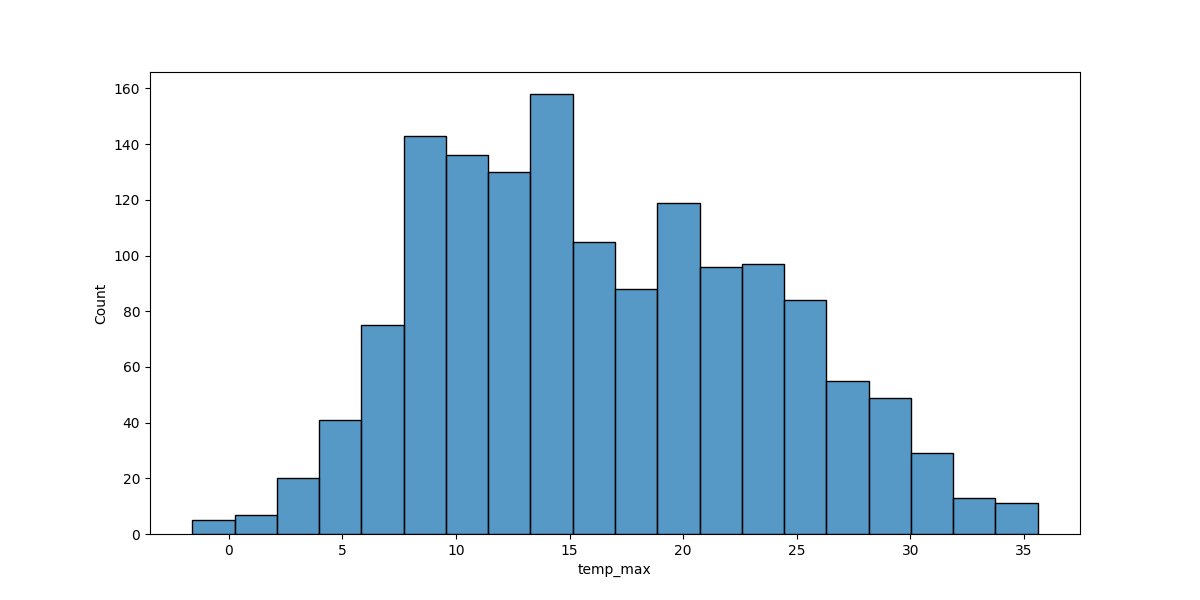
\includegraphics[width=\linewidth]{"Figures/Figure1.png"}
		\caption{Max. Sıcaklık Değeri Grafiği}
		\label{fig:ornek}
	\end{figure}
	
	Bu grafik, x ekseninde sıcaklık değerlerini ve y ekseninde bu sıcaklık değerlerine sahip olan gündüzlerin sayısını (COUNT parametresi) gösteriyor.
	
	\begin{figure}[h]
		\centering
		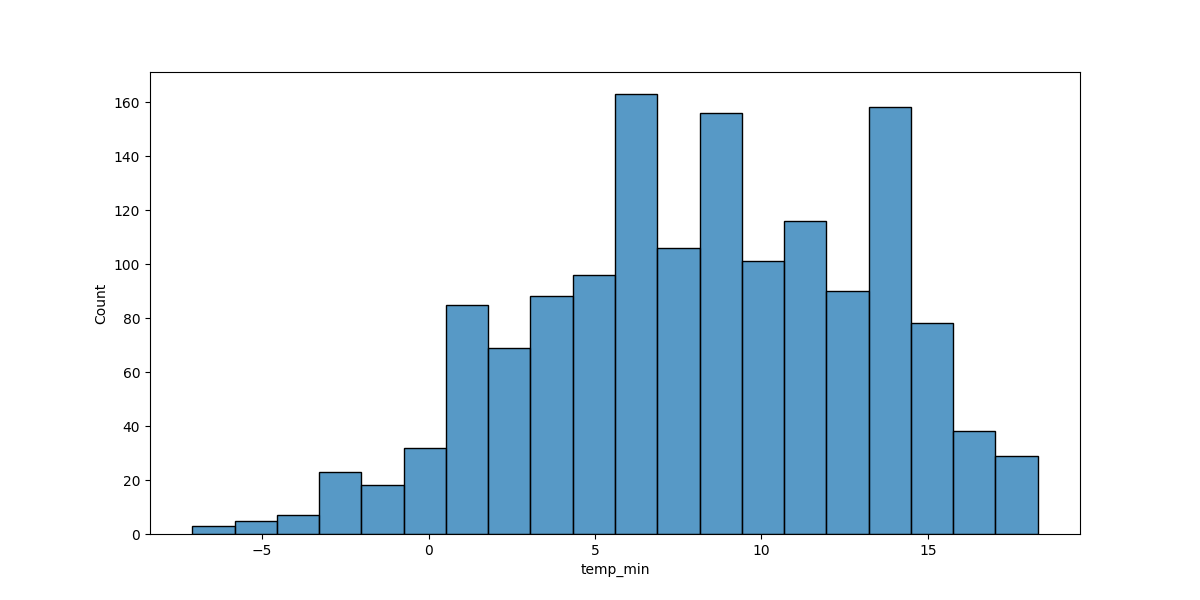
\includegraphics[width=\linewidth]{"Figures/Figure2.png"}
		\caption{Min. Sıcaklık Değeri Grafiği}
		\label{fig:ornek}
	\end{figure}
	
	Bu grafik, x ekseninde sıcaklık değerlerini ve y ekseninde bu sıcaklık değerlerine sahip olan gecelerin sayısını (COUNT parametresi) gösteriyor.
	
	\begin{figure}[h]
		\centering
		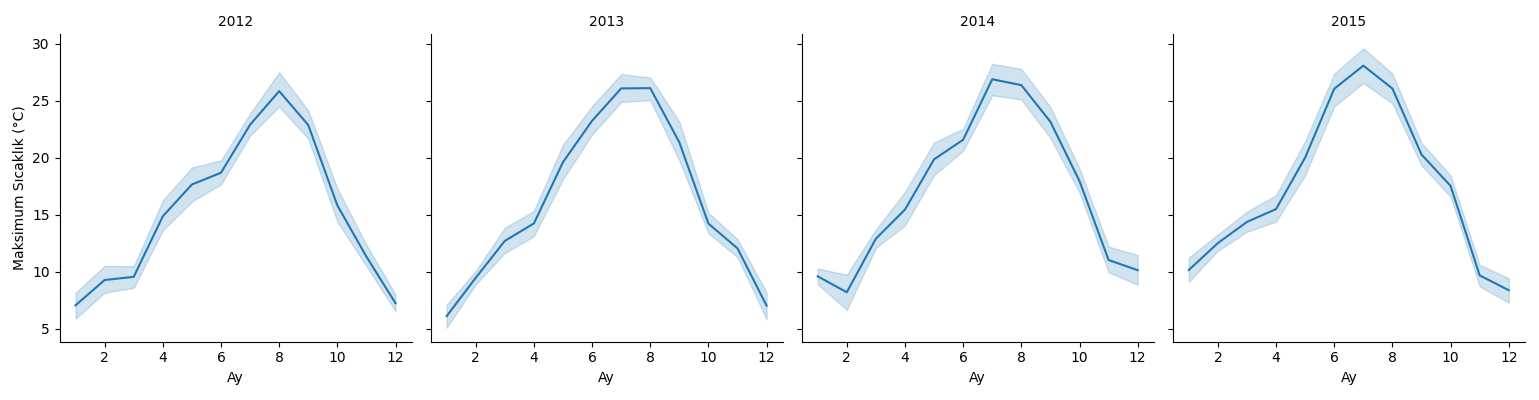
\includegraphics[width=\linewidth]{"Figures/Figure3.png"}
		\caption{Max. Sıcaklıklar Grafikleri (2012-2015)}
		\label{fig:ornek}
	\end{figure}
	
	Yukarıdaki grafiklerde, 2012-2015 yılları arasındaki ayların ortalama maksimum sıcaklık değerlerini göstermektedir. 
	
	\begin{figure}[H]
		\centering
		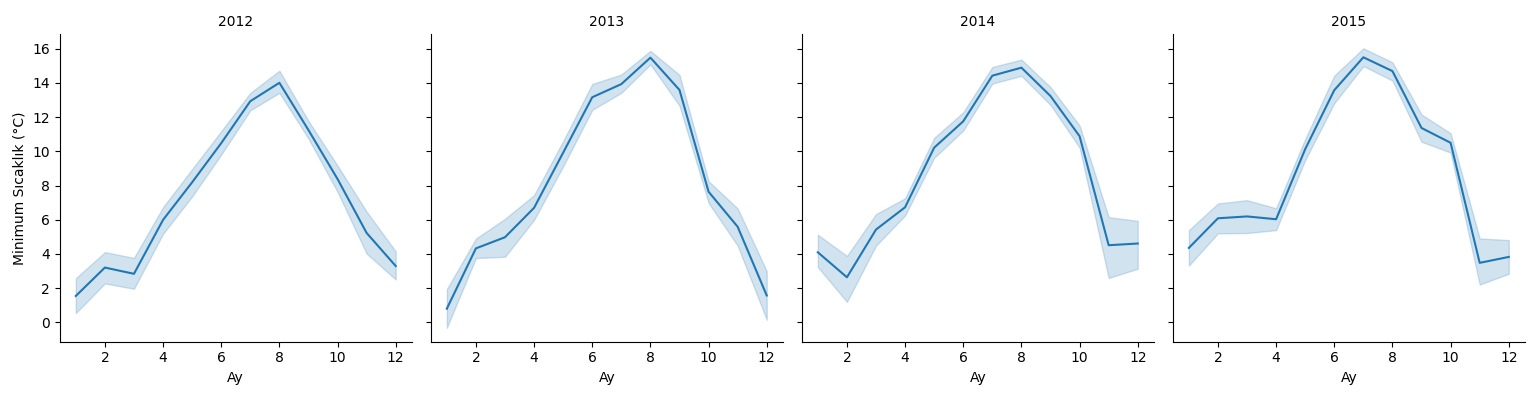
\includegraphics[width=\linewidth]{"Figures/Figure4.png"}
		\caption{Min. Sıcaklıklar Grafikleri (2012-2015)}
		\label{fig:ornek}
		
	\end{figure}
	Yukarıdaki grafiklerde, 2012-2015 yılları arasındaki ayların ortalama minimum sıcaklık değerlerini göstermektedir. 
	
	\begin{figure}[H]
		\centering
		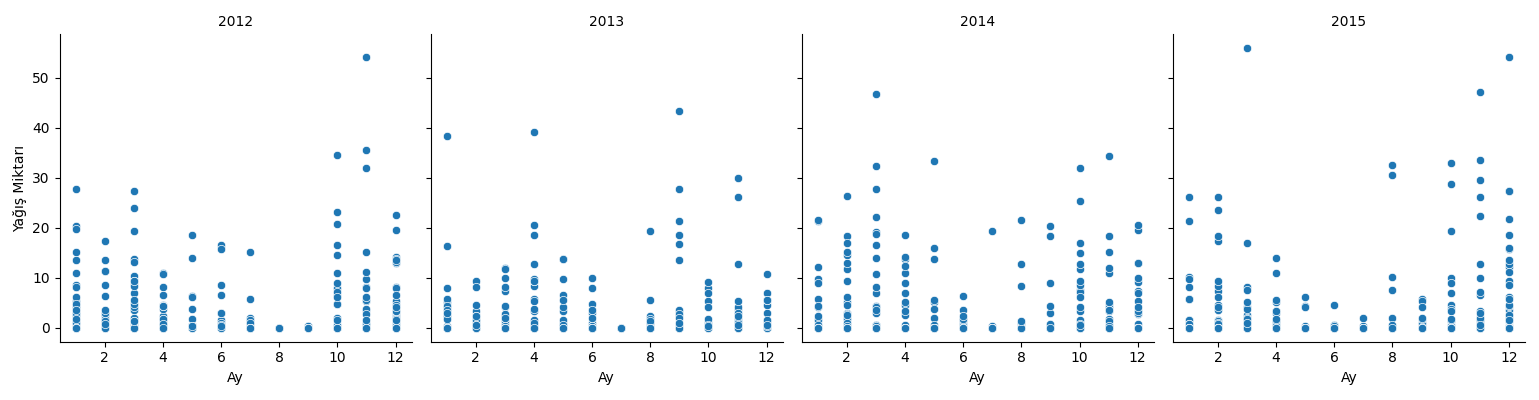
\includegraphics[width=\linewidth]{"Figures/Figure5.png"}
		\caption{Yağış Miktarı Grafikleri (2012-2015)}
		\label{fig:ornek}
	\end{figure}
	
	Yukarıdaki grafiklerde, 2012-2015 yılları arasındaki ayların yağış miktarları verilmiştir.
	
	\begin{figure}[h]
		\centering
		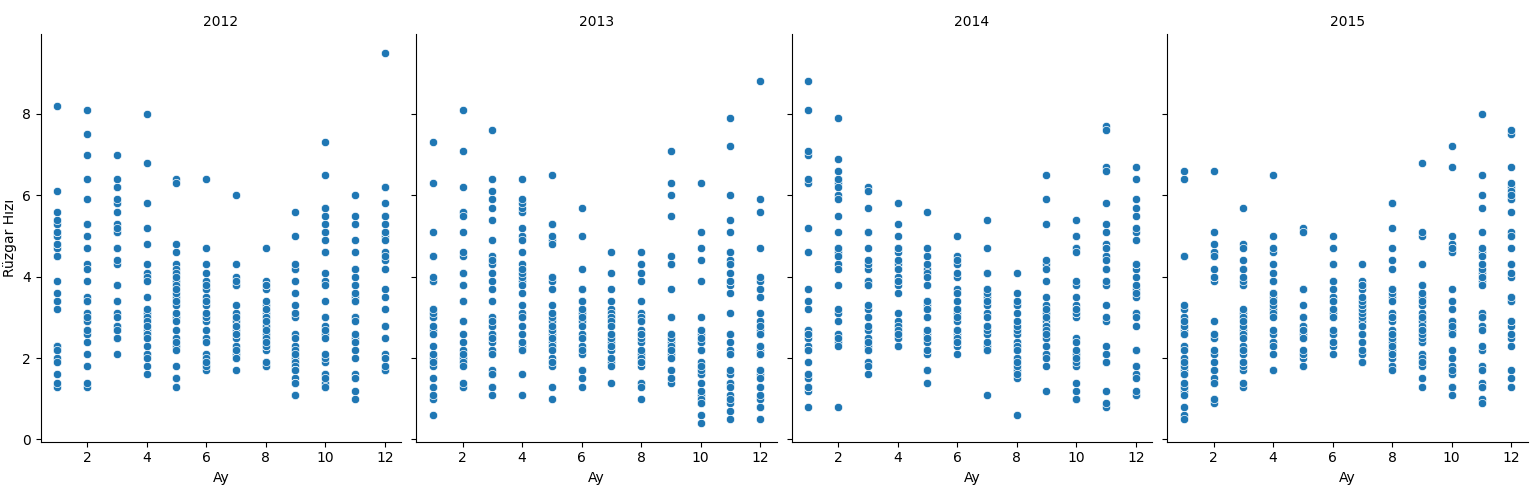
\includegraphics[width=\linewidth]{"Figures/Figure6.png"}
		\caption{Rüzgar Hızı Grafikleri (2012-2015)}
		\label{fig:ornek}
	\end{figure}
	
	Yukarıdaki grafiklerde, 2012-2015 yılları arasındaki aylarda rüzgarların hızları verilmiştir.
	
	\begin{figure}[h]
		\centering
		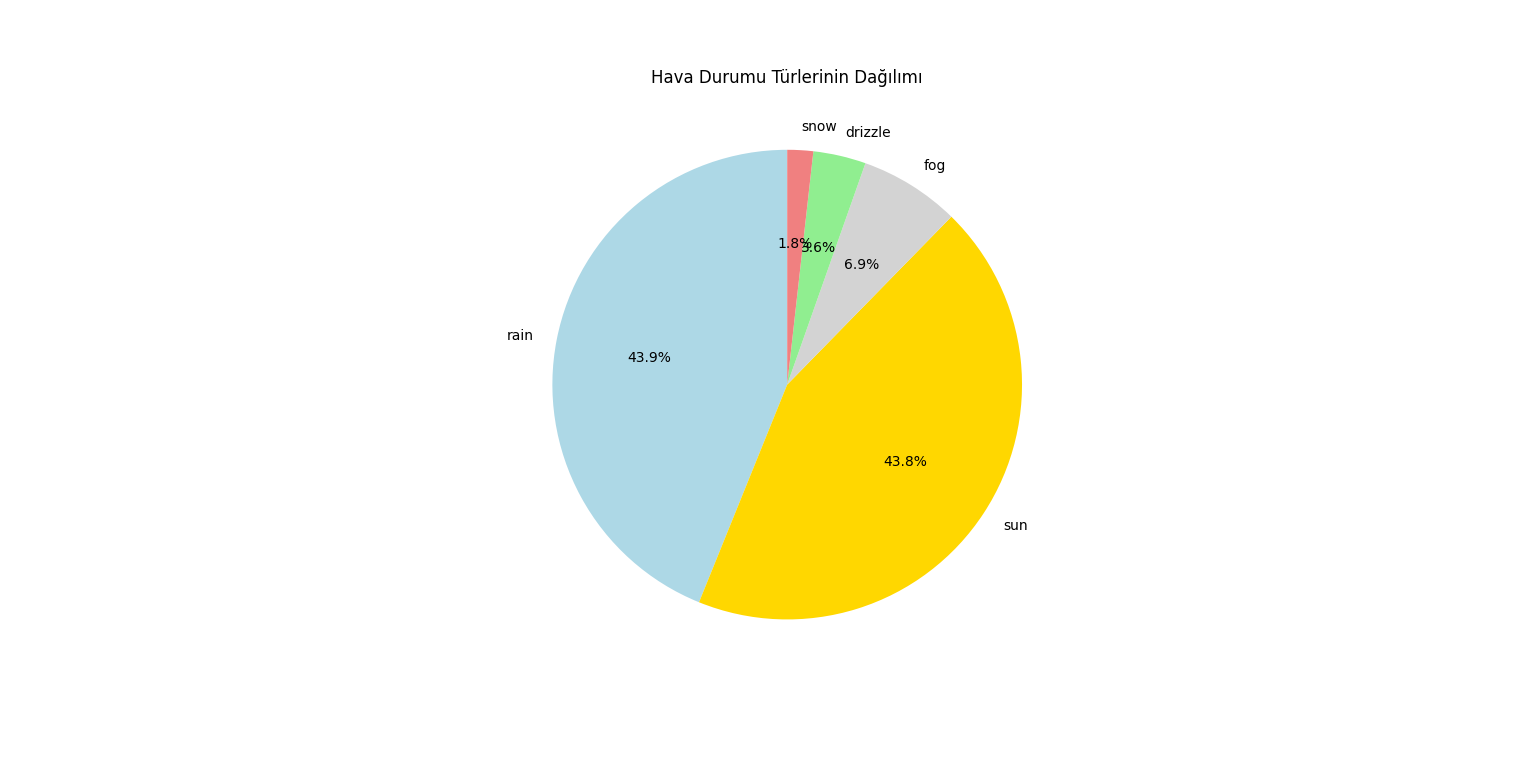
\includegraphics[width=\linewidth]{"Figures/Figure7.png"}
		\caption{Hava Durumu Türlerinin Dağılımları}
		\label{fig:ornek}
		
	\end{figure}
	Verilen dairesel grafikte hava durumu türlerinin (sun, rain, fog, snow, drizzle) dağılımları verilmiştir.
	Yıl boyunca güneşli ve yağmurlu günlerin sayısı diğer günlere oranla daha fazladır. En az görülen hava durumu ise karlıdır. 
	
	\begin{figure}[H]
		\centering
		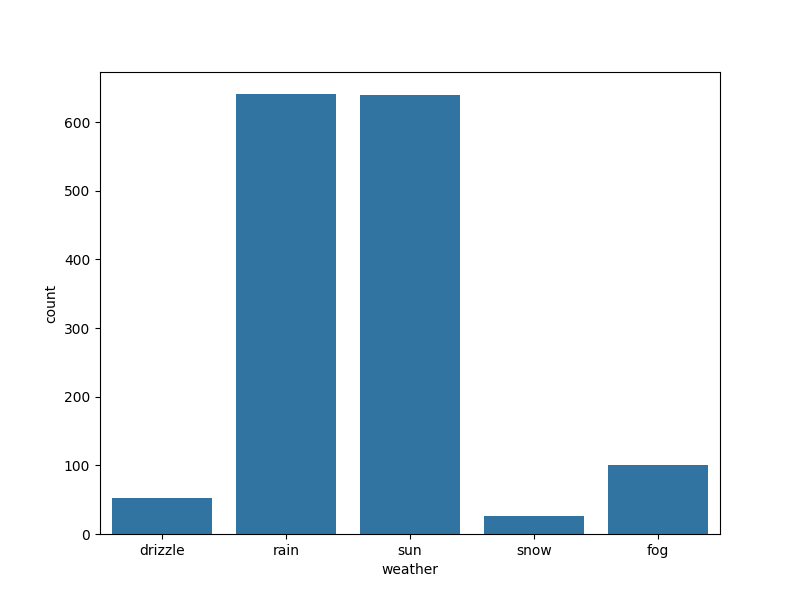
\includegraphics[width=\linewidth]{"Figures/Figure8.png"}
		\caption{Hava Durumu Türlerinin Tekrarlama Sıklığı}
		\label{fig:ornek}
		
	\end{figure}
	Verilen sütun grafiğinde, hava durumlarının (drizzle, rain, sun, snow, fog) 3 yıl içerisinde kaç defa tekrarlandığını göstermektedir. (Örneğin; yağmurlu gün sayısı 600'dür.)
	
	\section{BULGULAR}
	\subsection{Doğruluk Değerleri Tablosu}
	
	\begin{table}[h]
		\centering
		\resizebox{0.9\columnwidth}{!}{%
			\begin{tabular}{|l|c|c|}
				\hline
				\textbf{Model} & \textbf{CV Accuracy} & \textbf{F1 Score} \\ \hline
				GradientBoosting & 0.802 & 0.802 \\ \hline
				RandomForest & 0.788 & 0.789 \\ \hline
				DecisionTree & 0.753 & 0.752 \\ \hline
				LogisticRegression & 0.735 & 0.731 \\ \hline
				KNeighbors & 0.716 & 0.717 \\ \hline
				SVC & 0.700 & 0.708 \\ \hline
			\end{tabular}%
		}
		\caption{Model Performansı}
		\label{tab:model-performansi}
	\end{table}
	
	
	Tablo, çeşitli makine öğrenimi modellerinin performansını iki ana metrik kullanarak karşılaştırmaktadır: Cross-Validation Accuracy (Çapraz Doğrulama Doğruluğu) ve F1 Score (F1 Skoru). Her iki metrik de modelin ne kadar iyi performans gösterdiğini ölçer, ancak farklı yönlerden değerlendirirler.
	
	İşte her modelin performansını ve metriklerin ne anlama geldiğini açıklayan bir yorum:
	\begin{flushleft}
		\textbf{Metriğin Anlamı}
		
		\textbf{Cross-Validation Accuracy (Çapraz Doğrulama Doğruluğu):}
		Bu metrik, modelin doğruluğunu ölçer. Yani modelin, veriyi ne kadar doğru sınıflandırabildiğini gösterir. Çapraz doğrulama, veri setinin farklı bölümlerinde eğitim ve test işlemleri yaparak, modelin genel performansını daha güvenilir bir şekilde değerlendirmeyi sağlar.
		
		\textbf{F1 Score (F1 Skoru):}
		Bu metrik, modelin hassasiyet (precision) ve duyarlılık (recall) değerlerinin harmonik ortalamasıdır. Özellikle dengesiz veri setlerinde (yani bir sınıfın diğerine göre daha fazla veya az olduğu durumlarda) kullanışlıdır. Hem yanlış pozitifler hem de yanlış negatifler için ceza uygulayarak modelin genel performansını ölçer.
	\end{flushleft}
	
	\begin{flushleft}
		\textbf{MODELLERİN PERFORMANSI}
		
		\textbf{GradientBoostingClassifier:}
		\item Cross-Validation Accuracy: 0.802
		\item F1 Score: 0.802
		\item Yorum: Bu model, en yüksek doğruluğu ve F1 skorunu elde ederek diğer modellere göre en iyi performansı gösteriyor. Bu, modelin veriyi hem genel anlamda doğru sınıflandırdığını hem de sınıflar arasında dengeli bir performans sergilediğini gösterir.
		
		\textbf{RandomForestClassifier:}
		\item Cross-Validation Accuracy: 0.788
		\item F1 Score: 0.789
		\item Yorum: Bu model, Gradient Boosting'e çok yakın bir performans sergiliyor. Doğruluk ve F1 skorunun yüksek olması, modelin güvenilir ve dengeli olduğunu gösterir.
		
		\textbf{DecisionTreeClassifier:}
		\item Cross-Validation Accuracy: 0.753
		\item F1 Score: 0.752
		\item Yorum: Bu modelin performansı orta düzeyde. Karar ağaçları genellikle daha basit ve yorumlanabilir modellerdir, ancak doğruluk ve F1 skoru, daha karmaşık modellerin gerisinde kalıyor.
		
		\textbf{LogisticRegression:}
		\item Cross-Validation Accuracy: 0.735
		\item F1 Score: 0.731
		\item Yorum: Bu model, biraz daha düşük performans gösteriyor. Logistic Regression, özellikle lineer olarak ayrılabilir veriler için iyi çalışır, ancak bu veri setinde diğer modellerin gerisinde kalmış.
		
		\textbf{KNeighborsClassifier:}
		\item Cross-Validation Accuracy: 0.716
		\item F1 Score: 0.717
		\item Yorum: Bu modelin doğruluğu ve F1 skoru daha düşük. KNN, komşuluk tabanlı bir algoritma olduğu için büyük veri setlerinde veya yüksek boyutlu verilerde performansı düşebilir.
		
		\textbf{SVC (Support Vector Classifier):}
		\item Cross-Validation Accuracy: 0.700
		\item F1 Score: 0.708
		\item Yorum: SVC, en düşük performansı gösteren model. Doğru parametre ayarlamaları yapılmadığında performansı düşebilir, ancak belirli veri türleri ve problem türleri için güçlü bir model olabilir.
		
		\textbf{GENEL DEĞERLENDİRME}
		\item \textbf{En İyi Performans:} GradientBoostingClassifier ve RandomForestClassifier modelleri, yüksek doğruluk ve F1 skoru ile en iyi performansı gösteriyor. Özellikle Gradient Boosting, sınıflar arasında dengeli bir performans sağlıyor.
		\item \textbf{Orta Seviye Performans:} DecisionTreeClassifier ve LogisticRegression, daha düşük ancak kabul edilebilir bir performans sergiliyor. Karar ağaçları, açıklanabilirliğin önemli olduğu durumlar için tercih edilebilir.
		\item \textbf{Düşük Performans:} KNeighborsClassifier ve SVC, en düşük performansı gösteriyor. KNN'nin büyük ve yüksek boyutlu verilerde performansı düşerken, SVC'nin doğru ayar gerektirdiği görülüyor.
		
		
		
		\bibliographystyle{unsrt}
		\renewcommand\refname{Kaynakça}
		\bibliography{mybibfile}
		
	\end{flushleft}
	
	
	
	
	
	
	
	
	
	
	
	
	
	
	
	
	
	
	
	
	
	
	
	
\end{document}
